\documentclass{article}

% Language setting
% Replace `english' with e.g. `spanish' to change the document language
\usepackage[english]{babel}
\usepackage{subcaption}

% Set page size and margins
% Replace `letterpaper' with `a4paper' for UK/EU standard size
\usepackage[letterpaper,top=2cm,bottom=2cm,left=3cm,right=3cm,marginparwidth=1.75cm]{geometry}

% Useful packages
\usepackage{amsmath}
\usepackage{graphicx}
\usepackage[colorlinks=true, allcolors=blue]{hyperref}

\title{Quantifying the Impact of the COVID-19 Pandemic on Mental Health Searches Using Euclidean Distance, Granger’s Causality, and Regression}
\author{Anusha Dudella}

\begin{document}
\maketitle

\section{Abstract}
COVID-19 is a contagious disease caused by the virus, SARS-CoV-2. Since its introduction in Wuhan,
China in 2019, this virus has spread to over 213 countries worldwide and was most prevalent in the
United States. While related diseases and variants of COVID-19 are tracked via the CDC surveillance
systems, increases in mental health disorders are underestimated. According to the Kaiser Family
Foundation, concerns about mental health and substance abuse remain elevated three years after the
onset of the COVID-19 pandemic. As the topic of mental health is associated with stigma, individuals
generally use social media and Google searches to get information. I decided to establish a
relationship and predict Google search frequencies of mental health-related keywords based on the
number of COVID-19 cases. The objective of my research is to quantify the impact of the COVID-19
pandemic on the potential increase of these mental health-related keywords.

\section{Introduction}

The COVID-19 pandemic created havoc by resulting in the death of 7 million people worldwide.
COVID-19 resulted in several long-term physical effects like muscle pains, upper respiratory problems,
and fatigue. It also had a huge effect on people’s mental health and increased cases of disorders like
suicide, anxiety, depression, and drug overdose. As per the Centers for Disease Control, it is
estimated that about 50 million people are affected by mental health disorders of various kinds and
there has been a 35\% increase in mental health disorders cases from pre-COVID to post-COVID time.
It has always been the case that mental health disorder counts were very difficult to track as it is
difficult to recognize them distinctly unlike the physical symptoms.
With the rapid growth of the internet and the usage of Google searches, there have been many cases
where we predicted the emergence of pandemics or political unrest with that information. In this paper,
my goal is to find a correlation between the search frequencies of common mental health disorders
like depression, anxiety, anorexia, etc., and COVID-19 cases. With this correlation established, we can
say that COVID-19 cases caused a spike in the search frequency for mental health terms which can
be indicative of more mental health issues perceived by people.
To explore the impact of COVID-19 on mental health, I decided to analyze these three research
questions.
\\
\\Hypothesis I: COVID-19 increased Google searches for anorexia, depression, and anxiety in the
United States.
\\
\\Hypothesis II: COVID-19 increased Google searches for anorexia, depression, and anxiety more
in state A than in state B. (Oregon than Ohio)
\\
\\Hypothesis III: COVID-19 case trends are predictive of Google searches for ADHD in the US.

\section{Data}

\subsection{Datasets}

While there were many ways I could determine the relationship between mental health searches
and COVID-19 frequencies, I decided to go with the Google Trends database to get search
frequencies for a specific time period. An issue I encountered with this was that Google Trends
didn’t seem to have an API, so I relied on ‘Py-Trends,’ an open-source Python library that
provides its own measures for interacting with Google Trends data. Through Py-Trends, I was
able to extract data on keywords for different time periods and regions. For the COVID-19 case
data, I relied on COVID-19 time series data downloaded from the NY Times GitHub repository.

\subsection{Working with Sparse Data}

While I was experimenting with different keywords, time periods, and regions, I realized that I was
working with data that was ‘sparse’. For example, for NY region data, the frequency of the
keyword ‘anorexia’ returned zero search frequencies. This wasn’t realistic, as such a low
frequency for a common mental health disease in a state with a population of over seven million
wasn’t possible. I decided to filter out those specific regions, timeframes, or keywords that did not
give good data and focused on combinations of those that did.

\subsection{Data Wrangling}

The two datasets I was working with (NY Times and Google Trends) encapsulated different time
periods and were scaled differently. The Google Trends data were frequencies of keywords by week (weekly rolling averages) whereas the New York Times COVID data provided cases by day (daily rolling averages). Also, the Google Trends data was normalized to a scale of zero to
hundred whereas the New York Times COVID cases were the exact number of cases. To make
the data uniform, I wrote a program that compressed the daily rolling averages (from the New
York Times database) to weekly averages. I also used the min-max scaling algorithm to normalize
the actual counts to the same scale of data as Google Trends data.
\\
\\
\noindent Here is the formula used for normalization: \\
\\
\noindent $x^{\prime}=[x-\min (x)] /[\max (x)-\min (x)]$


\section{Hypothesis I - Time Series}

To determine whether COVID-19 increased the Google search frequencies for anorexia, depression,
and anxiety, I compared the data for the frequencies of search terms before COVID-19 (2018-2019)
and after COVID-19 (2020-2021). I then plotted this on a line graph to visualize the time series and
determine if there was an increase or not.

\begin{center}
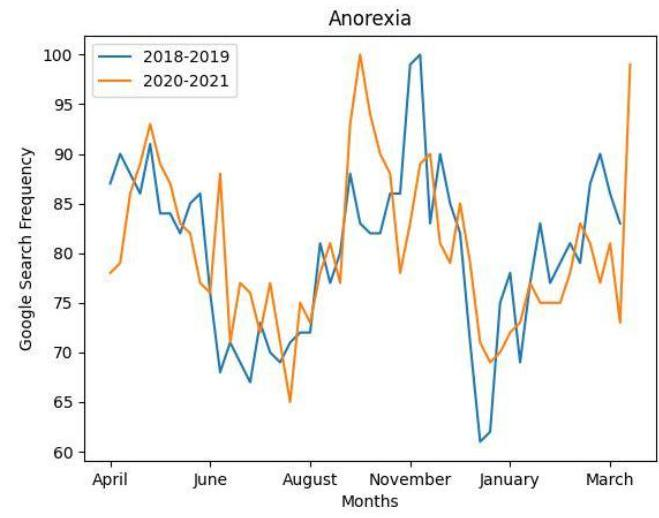
\includegraphics[scale=0.50]{2023_08_04_7b2b5ae1fb9d756e7758g-3}
\\ Figure 1a
\end{center}

\begin{center}
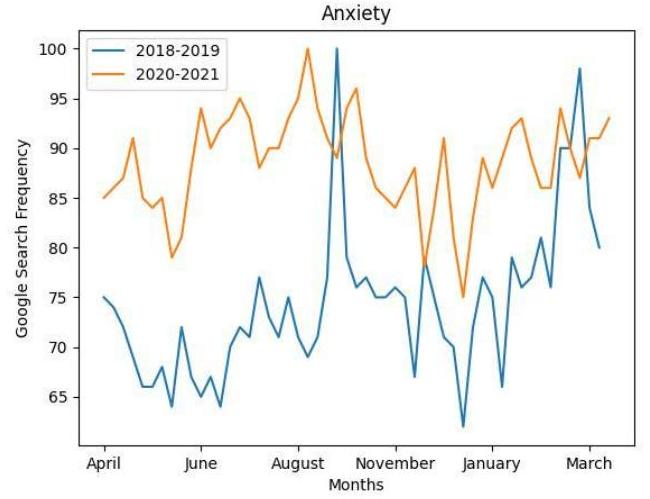
\includegraphics[scale=0.50]{2023_08_04_7b2b5ae1fb9d756e7758g-3(1)}
\\ Figure $1 b$
\end{center}

\begin{center}
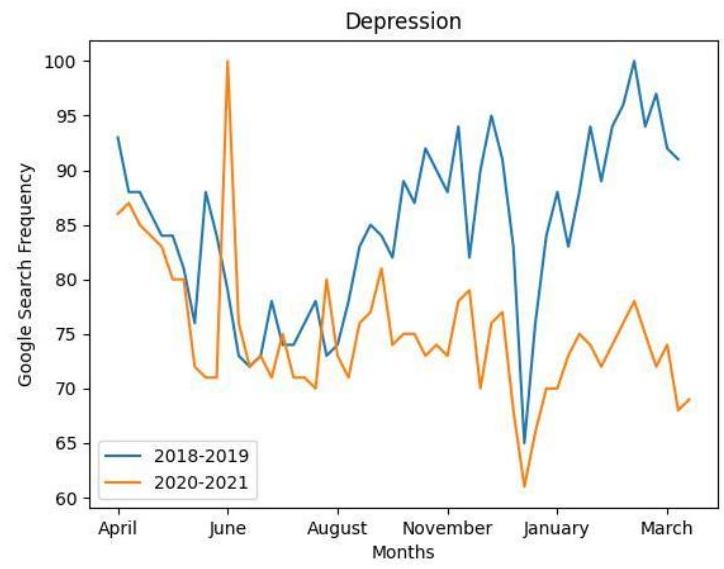
\includegraphics[scale=0.50]{2023_08_04_7b2b5ae1fb9d756e7758g-3(2)}
\\ Figure 1c
\end{center}

\subsection{Anorexia}

Figure 1a shows the Google search frequency for anorexia in the US had somewhat fluctuated for
both years. At the beginning of April 2020, the search frequency had been comparatively higher than
the 2018 graph. As time progresses, the 2020 graph seems to decrease and increase like the 2018
graph. There are a couple of months where the 2020-2021 graph seems to have more search
frequencies than 2018-2019, such as the spring-summer months. Towards the fall-winter seasons,
however, the 2018-2019 graph seems to have higher frequencies.

\subsection{Anxiety}

Figure 1b, shows that the Google search frequency for anxiety in the US had been significantly higher
in 2020-2021 than for 2018-2019. This coincides with my hypothesis that COVID-19 had increased the
frequency of the ‘Anxiety’ search term. Here, you can see that frequencies for ‘Anxiety’ had been
constantly higher for 2020-2021 compared to 2018-2019.

\subsection{Depression}

Figure 1c, shows the same type of seasonality as the first, with both the 2018-2019 and 2020-2021
graphs looking almost identical to each other. Besides 2020-2021 data being higher in frequencies for
a couple of months (mainly towards late Spring – early summer months), it seems that, overall, the
2018-2019 ‘depression’ keyword frequencies were higher than the 2020-2021 frequencies. We see
that from August to March, the Google search ‘depression’ frequencies for 2018-2019 are drastically
higher than the 2020-2021 Google search ‘depression’ frequencies.

\section{Hypothesis II - Euclidean Distance }

For hypothesis II, I worked with regional data (Oregon, Ohio, Texas, Colorado) that gave me “clean
data” and picked the exact three keywords (anorexia, depression, and anxiety) for each of these
states. I plotted each of these keywords for each state on a double-line graph for both years
2018-2019 and 2020-2021. Euclidean distance is a measure of how far apart the data is. The lower
the Euclidean distance value is, the more similar your data is for both timeframes and vice versa. I
then used Euclidean distance to find how the data for these two sets of years varied from each other. I
decided to analyze the state with the highest Euclidean distance value and the state with the lowest
Euclidean distance value so I could clearly see the disparity in results and determine whether the
COVID-19 increased Google searches for anorexia, depression, and anxiety more in State A than in
State B.
After experimenting with four different states that gave me a wide range of data, I selected Oregon and
Ohio is two states I was going to analyze before and after values of. This is because Oregon gave me
a higher Euclidean value for all keywords, signifying that it differed the most from its 2018-2019 to
2020-2021 values. I selected Ohio as the second state as it gave me the lowest Euclidean distance
value for all keywords, signifying that it differed the least from its 2018-2019 to 2020-2021 values.

\begin{center}
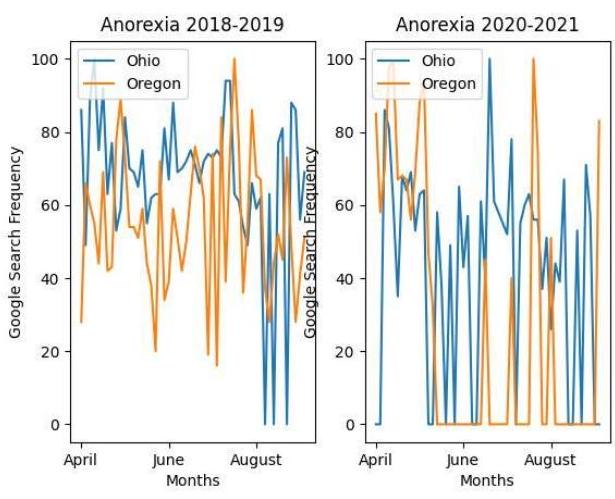
\includegraphics[scale=0.5]{2023_08_04_7b2b5ae1fb9d756e7758g-4}
\\ Figure 2a
\end{center}

\begin{center}
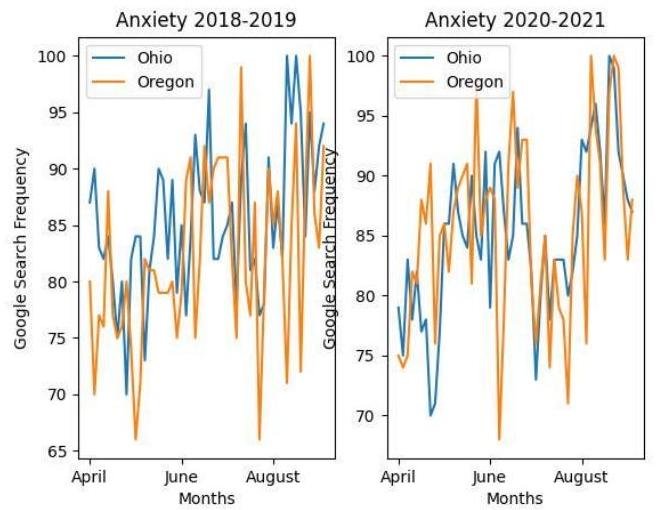
\includegraphics[scale=0.5]{2023_08_04_7b2b5ae1fb9d756e7758g-4(1)}
\\ Figure $2 b$
\end{center}

\begin{center}
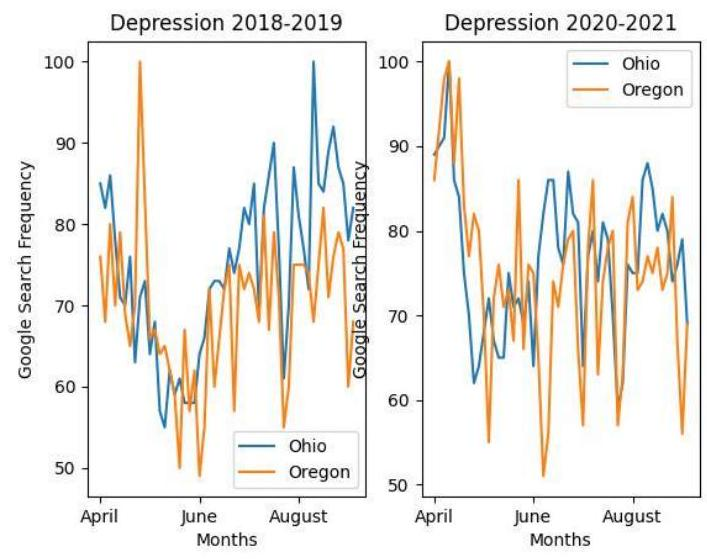
\includegraphics[scale=0.5]{2023_08_04_7b2b5ae1fb9d756e7758g-5}
\\ Figure $2 c$
\end{center}

\subsection{Anorexia}
In Figure 2a, the Euclidean distance for anorexia in Ohio (compared with both 2018-2019 to
2020-2021) value was 143.9. The Euclidean distance for Oregon (compared with both 2018-2019 to
2020-2021) was 359.469. Unexpectedly, when I was testing these keywords, I came across ‘sparse’
data. The graph above shows that the Google search frequencies, though scaled, did reach 0 for both
the 2018-2019 graph and the 2020-2021 graph. This shows that this data may not be accurate.

\subsection{Anxiety}
In Figure 2b, the Euclidean distance for anxiety in Ohio (compared with both 2018-2019 to 2020-2021)
values were 57.95. The Euclidean distance for Oregon (compared with both 2018-2019 to 2020-2021)
was 438.30. Looking at the graph, it is noticeable that the shape of the data for Oregon (for both time
periods) had changed more than the shape of the data for Ohio.

\subsection{Depression}
In Figure 2c, the Euclidean distance for depression in Ohio (compared with both 2018-2019 to
2020-2021) values were 72.09. The Euclidean distance for Oregon (compared with both 2018-2019 to
2020-2021) was 428.5. The shape of the graph of both years for Ohio seems to have changed a bit
more than anxiety, but the shape remains similar as compared to the Oregon graph, which seems to have
changed its shape dramatically over the two sets of time periods.

\section{Hypothesis III - Granger Causality and Linear Regression}
To determine whether COVID-19 case trends are predictive of Google searches for a mental health
keyword, I had to get a strong positive correlation between a specific keyword (from the timeframe:
2020-2021) and the COVID-19 case trends. A strong positive correlation is defined as a ‘correlation
coefficient above 0.5’ But, when I tested “anorexia” “depression” or “anxiety” with respect to the cases,
none of the keywords returned an R squared value above 0.5. After experimenting with multiple
different keywords and looking through the ‘Mental Health Center of America,’ I was able to find a mental
health keyword that returned a correlation above 0.5, ADHD.

\subsection{Granger Casuality}

The Granger Causality test is a statistical hypothesis test for determining whether one-time series is
useful for forecasting another time series. A time series of an independent variable (aka COVID
cases) is said to ‘Granger Cause’ Y through a series of T-hypothesis tests and that these X (COVID
cases) provide statistically significant information about the future values of Y. Subsequently, I
performed Granger’s Causality to establish whether there was a possibility that frequency
COVID-cases could cause the frequency of a keyword (ADHD). A null hypothesis suggests no
variance from the original hypothesis, signifying that there is “no variance.” On the other hand, an
alternative hypothesis signifies that there is a variance from the original hypothesis. A p-value is the
probability that your null hypothesis is true. A p-value of greater than 0.05 suggests that one “fails to
reject their null hypothesis” whereas a p-value of less than 0.05 suggests that one “rejects their null
hypothesis.” In this case, the null hypothesis I was testing is that the frequency of COVID cases does
not cause a frequency of ADHD searches. The alternative hypothesis would be that the frequency of
COVID cases do cause a frequency of ADHD searches. The Granger’s Causality test should return
a p-value from which I can conclude whether I can reject the null hypothesis or not.
\\
The null hypothesis for Hypothesis 3 is that COVID-19 case trends are not predictive of mental health
keywords (in this case, ADHD resulted in an R-squared value above 0.5). The alternative hypothesis is
that COVID-19 cases are predictive of mental health keywords (ADHD). If we look at US cases as our
X-variable and ADHD keyword search frequency as our Y-variable, it can be claimed that COVID-19
cases are predictive of the frequency of mental health keywords, as the p-value is 0.0.
\\
\noindent Below Figure 3a lists the values.

\begin{center}
\begin{tabular}{|l|l|l|}
\hline
\multicolumn{2}{|c|}{$\mathrm{p}$-value between ADHD and US Covid Cases} &  \\
\hline
 & ADHD & $\begin{array}{l}\text { US Covid } \\ \text { Cases }\end{array}$ \\
\hline
ADHD & 1.0 & 0.0 \\
\hline
$\begin{array}{l}\text { US Covid } \\ \text { Cases }\end{array}$ & 0.0001 & 1.0 \\
\hline
\end{tabular}
Figure 3a
\end{center}

\subsection{Linear Regression}
Linear Regression is used to model the relationship between two continuous variables. Often, the
objective is to predict the value of an output response based on the value of a predictor variable. In the
current setting, I used COVID cases in US as the independent or predictor variable and the search
term results for the term 'ADHD' as the output variable.
For this research, I gathered search term frequencies for the term 'ADHD' through, PyTrends, a
Python package that uses Google Trends API. I obtained COVID case counts for the entirety of the
US during the period of April 2020 through December 2022 and normalized the data.
I then split the data using Python scikit-learn utilities to give us about 50 weeks of test data from a total
of 150 weeks of data. I then trained the Linear Regression model with 100 weeks of training data and
predicted results for 50 weeks of test data. I utilized Python packages to calculate different metrics like
the mean, mean squared error, and the Root Mean Squared Error (RMSE).
RMSE value indicates how closely our predicted data reflects the test data. With our data set, I was
able to achieve a RMSE value of 4.4 indicating an approximate error of about 4.4 in our prediction
process. This means that the COVID cases count in the US could be used to predict the search
frequency of the mental health term, ADHD. Figure 4a below shows the predicted test vs actual test values (x and y respectively), and Figure 4b (also below) shows a residual plot that quantifies how far the actual-predicted values are from each other.

\begin{center}
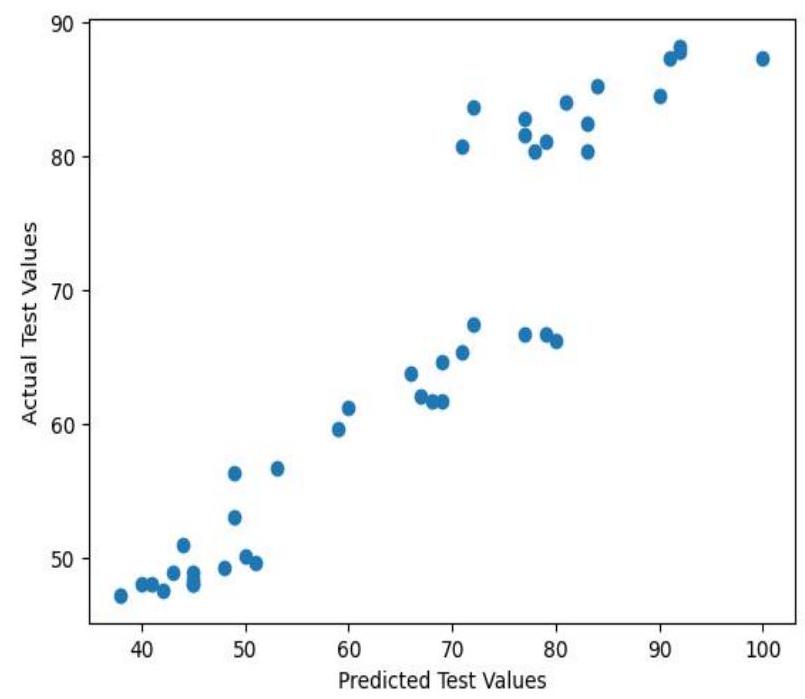
\includegraphics[scale=0.25]{2023_08_04_7b2b5ae1fb9d756e7758g-6}
\\Figure $3 b$
\end{center}



\begin{center}
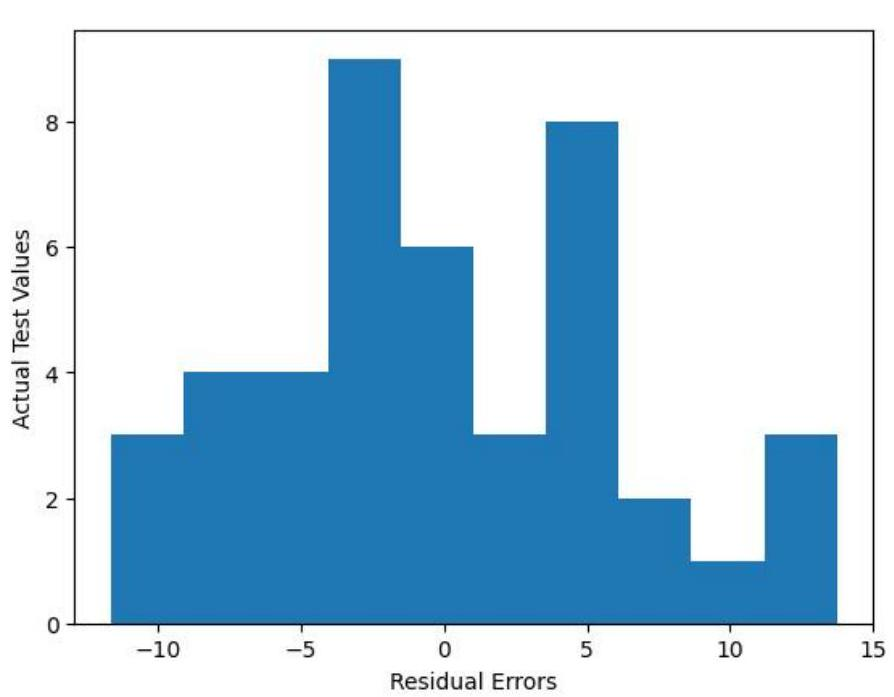
\includegraphics[scale=0.25]{2023_08_04_7b2b5ae1fb9d756e7758g-6(1)}
\\ Figure 3c
\end{center}

\section{Summary}
Through a longitudinal analysis of COVID-19 case data, keyword frequencies, and regions, I seemed
to have proved each of the hypotheses. Granted, I did have to experiment with the data, test keywords
that gave me a strong correlation, and clean up/invalidate data that did not seem to be of use.
\\With regards to Hypothesis I, I was able to establish that COVID-19 increased the frequency of the
mental health search term ‘anxiety’.
\\With regards to Hypothesis II, I was able to establish that COVID-19 increased the frequency of
search terms for ‘anorexia’ ‘anxiety’ and ‘depression in Oregon than in Ohio.
\\With regards to Hypothesis III, I was able to establish that COVID-19 trends are predictive of ADHD
search term interests in the US.

\section{Future Research}
In this paper, I have tried to establish a correlation between COVID-19 cases and the frequency of
search terms related to mental health disorders. I have taken a limited set of data from April 2020
through Dec 2022 to establish this relationship. In future research, we can continue to include the data
from the coming years to further establish a stronger correlation between these two topics. I have only
used US COVID-19 data to establish this correlation, but we can do the same analysis for other
countries and see if we can further strengthen our findings of a correlation between the two topics.
This research can be expanded to establish the relationship between several factors (like race,
economic status, and other existing health conditions) that impact the mental health of individuals. I
also believe that mental health disorders have a huge impact on the overall health of our society and if
we can in any way relate which among these factors are major contributors, it would be a huge
breakthrough.

\section{Acknowledgements}
I am very grateful to Dr. Mark Galassi, Mr. Mark Emry, and Ms.Rhonda Crespos for giving me this
opportunity to be part of this summer research internship at the Institute for Computing and Research.
I would like to express my sincere thanks to Dr. Sara Del Valle and Ms. Selina Hulley at the Los
Alamos National Laboratory for sharing their invaluable time, and knowledge, and guiding me through this
research. I would also like to thank the McNeil High School administration for hosting this summer
internship.

\section{Bibliography}
\begin{enumerate}
\item National Library of Medicine. "Controlling the COVID-19 pandemic: Useful lessons from Vietnam."NCBI, 10 July 2020, \href{https://www.ncbi.nlm.nih.gov/pmc/articles/PMC7347475/}{NCBI library}. Accessed 4 August 2023.

  \item Kaiser Family Foundation. "The Implications of COVID-19 for Mental Health and Substance Use." KFF, 20 March 2023, \href{https://www.kff.org/coronavirus-covid-19/issue-brief/the-implications-of-covid-19-for-mental-hea}{KFF article} Ith-and-substance-use/. Accessed 4 August 2023.

  \item WHO. WHO Coronavirus (COVID-19) Dashboard | WHO Coronavirus (COVID-19) Dashboard With Vaccination Data, \href{https://covid19.who.int/}{WHO COVID}. Accessed 4 August 2023.

  \item National Institute of Mental Health. "NIMH $»$ Mental Illness." NIMH, \href{https://www.nimh.nih.gov/health/statistics/mental-illness}{NIMH-Mental Health}. Accessed 4 August 2023.

  \item National Library of Medicine. "Covid and mental health in America - PMC." NCBI, 22 July 2022, \href{https://www.ncbi.nlm.nih.gov/pmc/articles/PMC9307159/}{National Library of Medicine}. Accessed 4 August 2023.

  \item NYT GitHub repo. "nytimes/covid-19-data: A repository of data on coronavirus cases and deaths in the U.S." GitHub, \href{https://github.com/nytimes/covid-19-data}{NY times}. Accessed 4 August 2023.

\end{enumerate}

\end{document}